\section{底层算子与计算成本}
\label{sec:operators}

\subsection{保持离散不变的算子边界}

非线性算子的输入是径向重构之后的各物理场角向半谱，输出是径向投影或有限差分右端构造之前的通量半谱。明确这一边界后，替换核必须从同一组重构系数计算同一去混叠乘积。减少真实时间样本、改变求积，或把弱通量形式改为另一种离散对流形式，都会改变数值方法，必须另外验收，不能被算子融合隐含地带入。

令 \(q\) 为该阶段的径向行数，\(N\) 为角向变换长度，\(H_N=\lfloor N/2\rfloor+1\) 为半谱宽度。数据按场优先排列，场 \(c\)、径向行 \(i\)、非负模态 \(k\) 的线性地址为 \(((cq+i)H_N+k)\)，每项保存一对 FP64 实虚部。Galerkin 读入 \(u_r,u_\theta,\omega\) 三个平面，返回 \(u_r\omega,u_\theta\omega\) 两个通量平面。FD 读入四个平面，返回两项导数乘积之和的一个平面；径向度量因子沿用原重构与右端约定。FD 的独立均值强迫由外部提供，仍按原角模升序相加。两条路径均在覆盖当前通量前，将原始通量复制到规定的 SBDF2 历史缓冲。

基线依次调用一次批量 cuFFT 逆变换、一个乘积核及一次批量 cuFFT 正变换。一个批量调用包含多个场和径向行，cuFFT 内部也可能启动多个设备核\cite{r11}。因此，三个高层操作不等于三个单场变换，更不等于性能分析器观测到的三个 GPU 节点。Galerkin 每行需要三个实逆变换和两个实正变换；FD 需要四个逆变换和一个正变换。二者均保留五个逻辑场变换。本节优化改变它们的实现方式。

\begin{figure}[!htbp]
\centering
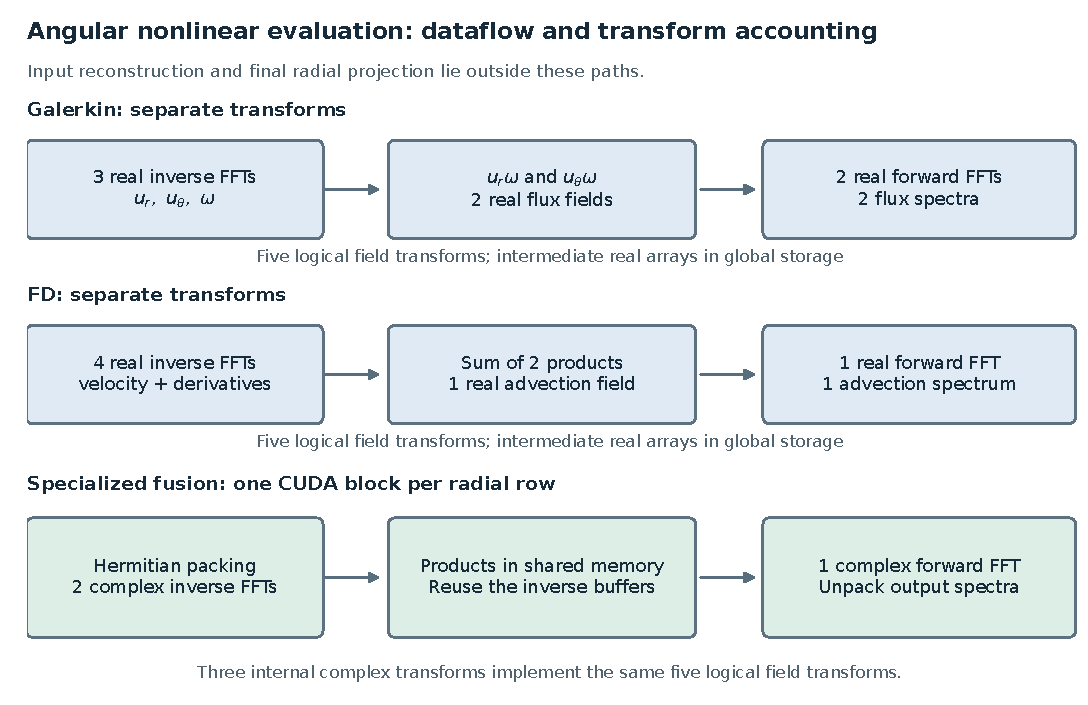
\includegraphics[width=\linewidth]{figures/nonlinear_pipeline.pdf}
\caption{非线性算子的替换边界。两种离散各自保留原有物理乘积。融合在共享内存中组织角向变换、点乘和打包；径向重构及投影位于图示替换范围之外。两种路径均保留五个逻辑场变换。}
\label{fig:operator-pipeline}
\end{figure}

\subsection{实场打包恒等式与归一化}

定义未归一化的正、逆离散 Fourier 变换为
\begin{equation}
\label{eq:op-dft}
(\mathcal F_N v)_k=\sum_{j=0}^{N-1}v_j e^{-2\pi\mathrm{i}jk/N},\qquad
(\mathcal B_N A)_j=\sum_{k=0}^{N-1}A_k e^{2\pi\mathrm{i}jk/N}.
\end{equation}
因此 \(\mathcal B_N\mathcal F_N=NI\)。CUDA 替换遵循 cuFFT 的符号及归一化约定\cite{r11}，不额外乘 \(1/N\)。求解器后续投影或 FD 右端已经包含相应尺度；若在两处同时归一化，即使单独的正逆变换测试看似正确，也会改变实际非线性方程。

对两个分别满足 Hermitian 对称的谱 \(A,B\)，由线性性可得
\begin{equation}
\label{eq:op-inverse-pack}
\mathcal B_N(A+\mathrm{i}B)=a+\mathrm{i}b,
\qquad a=\mathcal B_N A\in\mathbb R^N,\quad b=\mathcal B_N B\in\mathbb R^N.
\end{equation}
负模必须按 \(\overline{A_k}+\mathrm{i}\overline{B_k}\) 分别重建；若把整个打包正模共轭，则得到错误的 \(\overline{A_k}-\mathrm{i}\overline{B_k}\)。打包后的复谱通常不再满足 Hermitian 对称。零频和偶长度的 Nyquist 频率处，每个原实场谱的虚部须为零。

形成两个实乘积 \(g,h\) 后，令 \(Z=\mathcal F_N(g+\mathrm{i}h)\)，可恢复各自的谱：
\begin{equation}
\label{eq:op-forward-pack}
G_k=\frac{Z_k+\overline{Z_{-k}}}{2},\qquad
H_k=\frac{Z_k-\overline{Z_{-k}}}{2\mathrm{i}}.
\end{equation}
Galerkin 使用一次打包复逆变换重构两速度，一次逆变换重构涡量，一次打包复正变换恢复两个通量。FD 分别打包两速度和两导数，形成点积后作一次正变换。因此内部都执行三个复变换。这是实现层的计数恒等式，不能推出 \(5/3\) 的加速比：原 cuFFT 实变换已经利用 Hermitian 冗余，打包、置换、同步及额外指令均有成本。

保留带为 \(|k|\le K\) 时，二次乘积谱支撑至多为 \(2K\)。若别名进入保留模态，则存在非零整数 \(\ell\) 使 \(|k+\ell N|\le2K\)。而 \(|k+\ell N|\ge N-K\)，故严格条件 \(N>3K\) 排除了这一可能。这是经典的保留带去混叠论证\cite{r13}，并不表示乘积中不存在高于 \(K\) 的模态，也不能消除径向求积误差。替换核保持原角向填充长度和截断方式。

\subsection{线程映射、同步与访存}

每个径向行由一个128线程块处理，两块各含 \(N\) 个复双精度数的共享数组保存打包逆变换输入及物理场。专用长度及分解为 \(200=2^3 5^2\)、\(225=3^2 5^2\)、\(243=3^5\)，每块共享存储分别为6400、7200、7776字节。它们是明确实例化的长度，不是通用任意长度 FFT 服务。

设有序基数为 \(r_0,\ldots,r_{s-1}\)，将位置展开为混合进制数字 \(d_j\)，装载置换为
\begin{equation}
\label{eq:op-permutation}
p(i)=\sum_{j=0}^{s-1}d_j\frac{N}{\prod_{\ell=0}^{j}r_\ell},\qquad
i=\sum_{j=0}^{s-1}d_j\prod_{\ell=0}^{j-1}r_\ell.
\end{equation}
在前序基数积为 \(m\)、当前基数为 \(r\) 的阶段，各蝶形在乘旋转因子后合并间隔为 \(m\) 的位置。线程以128为跨度分配互不重叠的蝶形，相邻阶段之间执行全块屏障。这是经典混合基 FFT 构造；本项目的实现贡献在于它与当前算子边界及数据布局的结合，而非新的 FFT 分解。

完整执行顺序为：按置换装载两块打包逆变换平面，完成逆变换各阶段，各线程把一至两个物理乘积暂存寄存器，等待读取完成后覆盖第一块共享平面，执行正变换，拆包并写出半谱。寄存器暂存及覆盖前屏障必不可少，因为其他线程可能仍需读取原逆变换结果。即使全核只有一个线程块，省去该屏障仍会引入读写竞争。计入装载和覆盖屏障后，共有 \(2s+3\) 次全块同步，三种长度分别为13、11、13次。

原分离路径在全局内存中显式保存逆变换物理数组和正变换乘积数组。仅按这些命名数组的写入和读取计数，每次非线性评估名义消除 \(80Nq\) 字节访问：Galerkin 对应 \((3+3+2+2)Nq\) 个 double，FD 对应 \((4+4+1+1)Nq\) 个 double。这是这些实数组的源码级访问模型，并非设备总流量减少的上界；它未纳入缓存复用、编译器行为、库工作区，也不包含仍需保留的输入谱、输出谱及通量历史访问。因此它不是实测显存带宽数据，不能直接换算为速度增益。

融合同时增加共享存储、寄存器生命周期及单块工作量。径向行数较小时，线程块总数也可能不足以充分利用 GPU；消费级设备的 FP64 吞吐亦可能成为限制。由临时数组减少，不能直接判断最终算子受显存带宽、指令吞吐还是启动延迟限制。Roofline 或占用率结论需要本研究未采集的硬件计数器及受控测量。

\subsection{浮点边界与带保护的独立样例}

式~\eqref{eq:op-inverse-pack}--\eqref{eq:op-forward-pack}在精确算术下成立。浮点情况下，尺度为 \(A\) 的强通道可能向尺度为 \(B\) 的弱通道引入约 \(\epsilon A\) 量级的绝对扰动，对应相对尺度为 \(\epsilon A/B\)，还未计入变换常数和抵消。这是解释误差传播的尺度估计，并非该核的误差上界。它说明合并向量的相对误差很小，仍可能掩盖弱通道的相对误差；存在强抵消时，还需要按未抵消乘积大小缩放的绝对误差。

本次修订将原 CUDA 文件和既有 CPU 模型逐字提取，并新增不依赖求解器的验证入口及 NumPy、直接卷积参考。输入契约检查支持长度、连续 FP64 布局、实端点、零填充、有限数值及保留带宽。新增工程保护是：同一径向行内，若两个非零打包输入谱的最大模之比小于 \(10^{-8}\)，则默认拒绝执行。该阈值是保守的分派策略，不是保证相对精度的充分条件；严格为零的通道须采用绝对误差检查。真正的生产集成还需一个经验证的不打包后备路径，以及低成本获得尺度的方法；本样例没有宣称完成这些工作。冻结 NS 内核及其资格记录保持原状。

独立入口已在本机 GPU 完成36个固定态测试，覆盖三种长度、两种算子及每种算子六类输入。第六类在 Galerkin 中为一个速度通道严格为零，在 FD 中为两项相加抵消，因此两种算子合计使用七种不同标签。除独立 NumPy FFT 参考外，还使用不调用 FFT 的保留带多项式卷积参考，另验通量历史及 FD 均值缓冲奇偶位置。每输出通道的相对误差定义为跨径向行及半谱模态的无穷范数比 \(\max_{i,k}|Y_{ik}-Y^{\rm ref}_{ik}|/\max_{i,k}|Y^{\rm ref}_{ik}|\)，并非逐点相对误差。普通输入的各输出通道最大相对误差为 \(1.18\times10^{-15}\)。绝对误差诊断采用跨输出通道的统一尺度：对每行、每通量表达式，分别取各物理因子的最大模，将对应乘积相加并乘 \(N\)，最后在全部行和通道上取最大值。所有输入按此未抵消尺度缩放的最大绝对误差为 \(3.84\times10^{-16}\)；统一尺度可能掩盖弱通道误差，因此必须同时查看逐通道相对指标。将一个速度通道缩小到 \(10^{-10}\)，先确认保护拒绝，再显式放行作诊断后，单通道相对误差最大达到 \(4.98\times10^{-6}\)。这里采用向上取整的简写值，是新合成输入验证，不能替代原归档实测数字。本次提取未新增计时或 NS 轨迹，并以本地贡献候选的状态附于源码包。

\subsection{观测归约与 CPU 原生核}

探针算子计算六个加权和 \(p_j=w_j^\top x+\ell_j(t)\)。原实现让每个探针由一条线程串行处理；新实现为每个探针分配一个完整 warp，lane \(\ell\) 累加 \(\ell+32m\) 位置，再经五级 shuffle 归约合并\cite{r18}。一个192线程块覆盖全部六个探针。总算术工作仍与 frame 长度 \(L\) 线性相关，但每探针的串行深度由约 \(L\) 降为 \(\lceil L/32\rceil+5\)，这里没有把访存及指令成本视为零。快照复制、状态指针和推进前的同步均保留。求和次序改变会影响舍入，因此状态逐位不变与探针数值一致是两个独立检查。相应 Galerkin 与 FD 对照采用相同观测优化。

Python 驱动以下也有真实的项目内 C 实现。Galerkin 收缩核使角模成为连续内层维度，合并相同的预收缩质量与通量投影；FD 缓冲核应用已经装配好的窄径向模板，复用工作数组并就地形成物理乘积；另一个带状回代核用缓存的实 LAPACK 因子处理交错存储的复右端。FD 编译启用优化及 AVX2 支持，并关闭浮点乘加收缩，但编译选项本身不能证明 SIMD 利用率或加速。相应 CPU 变体仍调用 SciPy 的部分 FFT 或分解服务，并未修改其库源码和算法。

上述实现说明存在底层代码改动，但代码存在不等于完整求解已经通过隔离计时。同理，将 Python 调度语言整体替换为 Rust，不会直接减少设备 FFT 工作量、保留秩或编译核初始化成本。语言迁移应由实测宿主瓶颈或可复用接口需求驱动。本文区分循环和布局改动，以及导入、编译缓存、CUDA 图调度等运行时改动。

\subsection{完整成本、摊销条件与上游边界}

用于归因的成本分解为
\begin{equation}
\label{eq:cost}
\begin{aligned}
T_{\rm total}={}&T_{\rm start}+T_{\rm prepare}+N_{\rm nl}C_{\rm nl}\\
&+N_{\rm step}C_{\rm lin}+N_{\rm obs}C_{\rm obs}+T_{\rm finish}.
\end{aligned}
\end{equation}
各成本代表相位加权的有效量，并非假设每一步耗时相同。其中 \(C_{\rm lin}\) 不重复包含已经列出的非线性及观测开销。时间网格改动影响 \(N_{\rm nl},N_{\rm step}\)，融合影响 \(C_{\rm nl}\)，warp 归约影响 \(C_{\rm obs}\)，准备复用和缓存影响其他项。不能跨不相干测量直接相加收益，也不能重复计入同一成本。

若原固定执行中比例为 \(f\) 的部分获得局部加速比 \(s\)，理想整体界为 \([1-f+f/s]^{-1}\)。额外初始化成本会进一步缩小收益。更明确地，令 \(S_b,S_f\) 为基线和融合设置成本，\(B_b,B_f\) 为一份其余条件相同的重复工作成本；只有真实复用设置时，融合路径在 \(m\) 次重复后胜出才等价于
\begin{equation}
\label{eq:op-amortization}
m(B_b-B_f)>S_f-S_b.
\end{equation}
若每个新进程都重新构建或加载相关状态，设置就不是一次性成本，必须改写摊销模型。下一节的固定态事件测量及短轨迹结果说明，这一区分会改变结论。显式 PTX 缓存也不意味着驱动 JIT、模块加载、上下文、计划及进程启动成本全部消失。

完整求解时钟包含构造、编译或加载、传输、FFT 准备、图捕获、推进、观测、同步、下载和释放；新进程时钟再包含解释器启动、导入及规定监督开销。两者均不能由核事件替代。独立数值资格可以并发完成，但延迟比较须串行使用 GPU 并监测外部活动。CPU 总占用率不是同精度性能指标。

最后，源码审计识别到的是项目内应用核及库接口调用，没有发现已修改的 cuFFT、cuFFTDx、SciPy 或 LAPACK 借入源码。NVIDIA 已提供 FFT 融合与卷积示例，并包括 cuFFT 流水线及可选 LTO 回调的对照\cite{r17}。因此合理的上游方向是新增多场 FP64 的“逆变换、跨场乘积、正变换”示例，而非声称发明 FFT 融合或修复 cuFFT。提交仍需同等融合的 cuFFTDx 实现、批量 cuFFT 基线、相同精度和填充、首次及重复使用成本，以及脱离本机的干净构建。本地样例尚不满足这些性能与可移植性条件，也未建立新的许可证授权或贡献签署，尚未提交 PR\cite{r19}。
